%%%%%%%%%%%%%%%%%%%%%%%%%%%%%%%%%%%
%This is the LaTeX ARTICLE template for RSC journals
%Copyright The Royal Society of Chemistry 2016
%%%%%%%%%%%%%%%%%%%%%%%%%%%%%%%%%%%

\documentclass[twoside,twocolumn,9pt]{article}
\usepackage{extsizes}
\usepackage[super,sort&compress,comma]{natbib} 
\usepackage[version=3]{mhchem}
\usepackage[left=1.5cm, right=1.5cm, top=1.785cm, bottom=2.0cm]{geometry}
\usepackage{balance}
\usepackage{mathptmx}
\usepackage{sectsty}
\usepackage{graphicx} 
\usepackage{lastpage}
\usepackage[format=plain,justification=justified,singlelinecheck=false,font={stretch=1.125,small,sf},labelfont=bf,labelsep=space]{caption}
\usepackage{float}
\usepackage{fancyhdr}
\usepackage{fnpos}
\usepackage[english]{babel}
\addto{\captionsenglish}{%
  \renewcommand{\refname}{Notes and references}
}
\usepackage{array}
\usepackage{droidsans}
\usepackage{charter}
\usepackage[T1]{fontenc}
\usepackage[usenames,dvipsnames]{xcolor}
\usepackage{setspace}
\usepackage[compact]{titlesec}
\usepackage{hyperref}
%%%Please don't disable any packages in the preamble, as this may cause the template to display incorrectly.%%%
\usepackage{mathtools}
\usepackage[version-1-compatibility]{siunitx}
\usepackage{enumitem}
\usepackage[referable]{threeparttablex}
\renewlist{tablenotes}{enumerate}{1}
\makeatletter
\setlist[tablenotes]{label=\tnote{\alph*},ref=\alph*,itemsep=\z@,topsep=\z@skip,partopsep=\z@skip,parsep=\z@,itemindent=\z@,labelindent=\tabcolsep,labelsep=.2em,leftmargin=*,align=left,before={\footnotesize}}
\makeatother
\newcommand{\ra}[1]{\renewcommand{\arraystretch}{#1}}
\usepackage{diagbox}
\usepackage{multirow}


%\usepackage{epstopdf}%This line makes .eps figures into .pdf - please comment out if not required.

\definecolor{cream}{RGB}{222,217,201}

\begin{document}

\pagestyle{fancy}
\thispagestyle{plain}
\fancypagestyle{plain}{
%%%HEADER%%%
\renewcommand{\headrulewidth}{0pt}
}
%%%END OF HEADER%%%

%%%PAGE SETUP - Please do not change any commands within this section%%%
\makeFNbottom
\makeatletter
\renewcommand\LARGE{\@setfontsize\LARGE{15pt}{17}}
\renewcommand\Large{\@setfontsize\Large{12pt}{14}}
\renewcommand\large{\@setfontsize\large{10pt}{12}}
\renewcommand\footnotesize{\@setfontsize\footnotesize{7pt}{10}}
\makeatother


\renewcommand{\thefootnote}{\fnsymbol{footnote}}
\renewcommand\footnoterule{\vspace*{1pt}% 
\color{cream}\hrule width 3.5in height 0.4pt \color{black}\vspace*{5pt}} 
\setcounter{secnumdepth}{5}

\makeatletter 
\renewcommand\@biblabel[1]{#1}            
\renewcommand\@makefntext[1]% 
{\noindent\makebox[0pt][r]{\@thefnmark\,}#1}
\makeatother 
\renewcommand{\figurename}{\small{Fig.}~}
\sectionfont{\sffamily\Large}
\subsectionfont{\normalsize}
\subsubsectionfont{\bf}
\setstretch{1.125} %In particular, please do not alter this line.
\setlength{\skip\footins}{0.8cm}
\setlength{\footnotesep}{0.25cm}
\setlength{\jot}{10pt}
\titlespacing*{\section}{0pt}{4pt}{4pt}
\titlespacing*{\subsection}{0pt}{15pt}{1pt}
%%%END OF PAGE SETUP%%%

%%%FOOTER%%%
\fancyfoot{}
\fancyfoot[LO,RE]{\vspace{-7.1pt}
\includegraphics[height=9pt]{head_foot/LF}}
\fancyfoot[CO]{\vspace{-7.1pt}\hspace{11.9cm}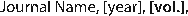
\includegraphics{head_foot/RF}}
\fancyfoot[CE]{\vspace{-7.2pt}\hspace{-13.2cm}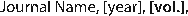
\includegraphics{head_foot/RF}}
\fancyfoot[RO]{\footnotesize{\sffamily{1--\pageref{LastPage} ~\textbar  \hspace{2pt}\thepage}}}
\fancyfoot[LE]{\footnotesize{\sffamily{\thepage~\textbar\hspace{4.65cm} 1--\pageref{LastPage}}}}
\fancyhead{}
\renewcommand{\headrulewidth}{0pt} 
\renewcommand{\footrulewidth}{0pt}
\setlength{\arrayrulewidth}{1pt}
\setlength{\columnsep}{6.5mm}
\setlength\bibsep{1pt}
%%%END OF FOOTER%%%

%%%FIGURE SETUP - please do not change any commands within this section%%%
\makeatletter 
\newlength{\figrulesep} 
\setlength{\figrulesep}{0.5\textfloatsep} 

\newcommand{\topfigrule}{\vspace*{-1pt}% 
\noindent{\color{cream}\rule[-\figrulesep]{\columnwidth}{1.5pt}} }

\newcommand{\botfigrule}{\vspace*{-2pt}% 
\noindent{\color{cream}\rule[\figrulesep]{\columnwidth}{1.5pt}} }

\newcommand{\dblfigrule}{\vspace*{-1pt}% 
\noindent{\color{cream}\rule[-\figrulesep]{\textwidth}{1.5pt}} }

\makeatother
%%%END OF FIGURE SETUP%%%

\newcommand{\pp}{\textcolor{blue}}
\newcommand{\sk}{\textcolor{cyan}}
\newcommand{\agsof}{\textcolor{green}}

%%%TITLE, AUTHORS AND ABSTRACT%%%
\twocolumn[
  \begin{@twocolumnfalse}
{
\includegraphics[height=30pt]{head_foot/PCCP}\hfill\raisebox{0pt}[0pt][0pt]{
\includegraphics[height=55pt]{head_foot/RSC_LOGO_CMYK}}\\[1ex]

\includegraphics[width=18.5cm]{head_foot/header_bar}}\par
\vspace{1em}
\sffamily
\begin{tabular}{m{4.5cm} p{13.5cm} }


\includegraphics{head_foot/DOI} & \noindent\LARGE{\textbf{Protocol for Optical Pumping of $\mathrm{AlH}^+$ to a Single Hyperfine State in the Ground Rovibronic Manifold}} \\%Article title goes here instead of the text "This is the title"
\vspace{0.3cm} & \vspace{0.3cm} \\

 & \noindent\large{Panpan Huang,\textit{$^{a}$} Schuyler Kain,\textit{$^{a}$} Antonio G. S. de Oliveira-Filho,\textit{$^{b}$}} and Brian Odom$^{\ast}$\textit{$^{a}$} \\%Author names go here instead of "Full name", etc.

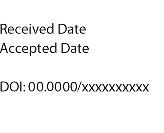
\includegraphics{head_foot/dates} & \noindent\normalsize{In this work, we propose an optical pumping scheme to prepare trapped $\mathrm{AlH}^+$ molecules in the stretched hyperfine state $\lvert F=\frac{7}{2},\, m_F=\frac{7}{2}\rangle$ of the rovibronic ground state $\lvert \mathrm{X}^2\Sigma^+,\, v=0,\, N=0\rangle$. Our scheme utilizes linearly-polarized and circularly-polarized fields of a broadband pulsed laser to cool the rotational degree of freedom and drive the population to the stretched hyperfine state, respectively. We find that adding a laser to couple the $v=1$ \pp{--} $v=0$ transition in the $ \mathrm{X}^2\Sigma^+$ state accelerates the cooling process. We conducted a simulation of the population dynamics by solving a representative system of rate equations. The hyperfine constants were also calculated to model the hyperfine structure. The results show that under optimum conditions, the population in the stretched hyperfine state of the rovibronic ground state can reach 63 $\%$ after 67.6 \si{\micro}s (334.6 ms) and 95 $\%$ after 25.4 ms (1.240 s) with (without) the rovibrational coupling laser.} \\%The abstrast goes here instead of the text "The abstract should be..."

\end{tabular}

 \end{@twocolumnfalse} \vspace{0.6cm}
]
%%%END OF TITLE, AUTHORS AND ABSTRACT%%%

%%%FONT SETUP - please do not change any commands within this section
\renewcommand*\rmdefault{bch}\normalfont\upshape
\rmfamily
\section*{}
\vspace{-1cm}


%%%FOOTNOTES%%%

\footnotetext{\textit{$^{a}$Department of Physics and Astronomy, Northwestern University, Evanston, IL 60208, USA.  E-mail: b-odom@northwestern.edu}}
\footnotetext{\textit{$^{b}$Departamento de Química, Laboratório Computacional de Espectroscopia e Cinética, Faculdade de Filosofia, Ciências e Letras de Ribeirão Preto, Universidade de São Paulo, Ribeirão Preto-SP 14040-901, Brazil. }}

%Please use \dag to cite the ESI in the main text of the article.
%If you article does not have ESI please remove the the \dag symbol from the title and the footnotetext below.

%additional addresses can be cited as above using the lower-case letters, c, d, e... If all authors are from the same address, no letter is required
%%%END OF FOOTNOTES%%%

%%%MAIN TEXT%%%%
\begin{figure*}[!htp]
 \centering
 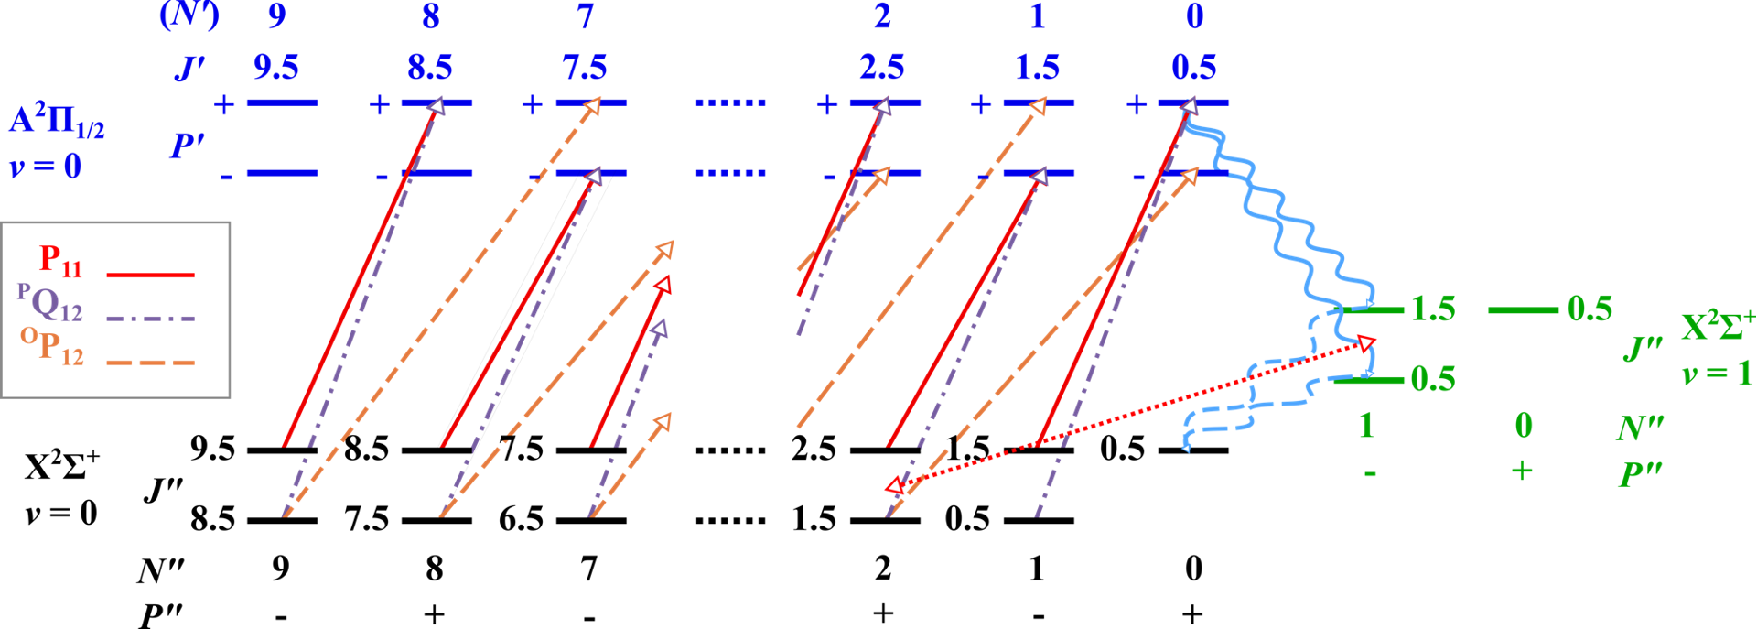
\includegraphics[width=14cm]{level_diagram_parity}
 \caption{\pp{Energy level structure} of $\mathrm{AlH}^+$ and the rotational cooling scheme. The rotational cooling laser drives $\mathrm{P_{11}}$, $\mathrm{^PQ_{12}}$ and $\mathrm{^OP_{11}}$ branches from $\lvert \mathrm{X}^2\Sigma^+, v=0\rangle$ to $\lvert \mathrm{A}^2\Pi_{1/2}, v=0\rangle$. Though the rotational angular momentum is not a good quantum number in $\mathrm{A}^{2}\Pi$, $N'$ is used here as a convenient label for different J values and transition branches. The time scale of the electronic relaxation without vibrational excitation from $\lvert \mathrm{A}^2\Pi_{1/2}, v=0\rangle$ to $\lvert \mathrm{X}^2\Sigma^+, v=0\rangle$ is around 0.4 \si{\micro}s. The solid wavy blue arrows represent the electronic spontaneous relaxation with vibrational excitation. The dashed wavy blue arrows represent the rovibrational relaxation within the $\mathrm{X}$ state, \pp{which happens on the time scale of 140 ms}. The rate of population transfer from $v=1$ to $v=0$ in the $\mathrm{X}$ state is then limited by this time scale, which can be decreased by adding the rovibrational coupling laser, denoted by V10 laser (indicated by the dashed red arrow).}
 \label{level_diagram_parity}
\end{figure*}

\section{Introduction}
%applicaitons
In recent years, molecules have played increasingly important roles in many active areas of research such as precision measurement\cite{kobayashi2019measurement, andreev2018improved, biesheuvel2016probing}, quantum simulation\cite{ohmori2017special}, quantum information processing\cite{grandstrand:2004, soderberg2009ultracold} and cold chemistry\cite{balakrishnan2016perspective, bohn2017cold}. \pp{For example, new physics may be revealed through the variations in the proton-to-electron mass ratio, $m_\mathrm{p}/m_\mathrm{e}$. The change of the transition frequency caused by the variation can be enhanced utilizing the nature of sensitivity difference in two internal states of molecules.\cite{demille2008enhanced, kobayashi2019measurement, kokish2018prospects, stollenwerk2018optical}} The measurement of the current upper limit of the electric dipole moment (EDM) of the electron today used polar molecules\cite{andreev2018improved} since \pp{they could have larger internal electric fields compared to those of atoms}. The rich internal degrees of freedom and the long-range dipole-dipole interaction between polar molecules also offer possibilities of developing a quantum toolkit for both quantum simulation and quantum information processing\cite{wei2011entanglement}. Furthermore, the chemical interaction process may be fundamentally controlled by preparing the external and internal states of the reactants\cite{de2011controlling}. These applications typically study isolated ensembles of molecules and employ various traps to achieve long interrogation times. Sometimes the measurement or interaction process is irreversible and new ensembles must be quickly prepared in the same initial state to achieve precision or statistical significance. \pp{Therefore, having the ability of fast repeatedly preparing molecules to a pure initial quantum state is essential in these applications.}\par

%In precision measurement, precise determination of certain transition frequencies by repeatedly driving those transitions is required. 
%In quantum simulation, quantum information processing and quantum chemistry, molecules may be required to populate certain pure internal states to exploit the state properties. 

Ion traps are one class of trap that is frequently employed. The deep \pp{trap} depth of ion traps is attractive because it suppresses the loss of trap population due to collisions with background gas. Trapped molecular ions are often sympathetically cooled with co-trapped Doppler-cooled atomic ions, leading to longer trapping lifetimes. Therefore, trapped molecular ions are well-suited for applications requires long interrogation time. The controlled cooling of the population in certain hyperfine states of the molecular ion, HD$^+$ has been previously demonstrated\cite{bressel2012manipulation}. Rotational cooling was accomplished by optically pumping selected rovibrational transitions\cite{schneider2010all}. Manipulation of the population at the hyperfine level was then performed by coupling individual hyperfine states within the pumped rovibrational levels. This hyperfine population transfer process took a few tens of seconds to increase the population of a chosen hyperfine state by a few percent.\par
%Ours
Our group has previously shown that rotational cooling of diatomic molecules can be achieved using a spectrally-filtered femtosecond laser (SFFL) with species that have relatively large rotational constants and fairly diagonal Frank-Condon factors (FCFs)\cite{lien2011optical}. One such example is aluminum monohydride cation, $\mathrm{AlH}^+$, for which we demonstrated an increase in the rotational ground state population from a few percent to $\sim$ 95 $\%$ within a second \cite{lien2014broadband}. Cooling to a single $M_{J}$ level was also theoretically investigated using the approach of optimal control theory \cite{aroch2018optimizing}. However, the operation of cooling $\mathrm{AlH}^+$ to a specified hyperfine state has not yet been addressed. $\mathrm{AlH}^+$ has one unpaired electron ($S=\frac{1}{2}$), and nuclei with nuclear spins $I_\mathrm{Al}=\frac{5}{2}$ and $I_\mathrm{H}=\frac{1}{2}$. The theory of angular momentum permits us to describe the hyperfine states of \pp{the electronic ground state of $\mathrm{AlH}^+$} in terms of \pp{a set of} angular momentum quantum numbers, where $\left\lbrace F \right\rbrace$ are total angular momentum quantum numbers, $J\left(=N+S\right)$ is the quantum number of the total angular momentum exclusive of nuclear spin, N is the molecular rotational quantum number, and S is the total electron-spin quantum number. We further define the members of the set of total angular momentum quantum numbers: $F_{1}=J+I_\mathrm{Al}$, and $F=F_{1}+I_\mathrm{H}$. Finally, we define the vibrational state through $v$, the vibrational quantum number. In its rovibronic ground state ($\mathrm{X}$, $v=0$, $N=0$), $\mathrm{AlH}^+$ has four hyperfine states: $F=\left\lbrace\frac{3}{2},\, \frac{5}{2}\right\rbrace$ for $F_{1}=2$ and $F=\left\lbrace\frac{5}{2},\, \frac{7}{2}\right\rbrace$ for $F_{1}=3$.\par

%In the rovibronic state ($N=0$), since $J=N+S$, $F_{1}=J+I_{1}$, $F=F_{1}+I_{2}$, AlH$^{+}$ has four hyperfine states which are $F=\frac{3}{2},\, \frac{5}{2}$ states for $F_{1}=2$ and $F=\frac{5}{2},\, \frac{7}{2}$ states for $F_{1}=3$.\par

\pp{The aim of this paper is to propose an efficient method to transfer the $\mathrm{AlH}^+$ population to a single stretched hyperfine state of the rovibronic ground state.} \pp{The paper is laid out as follows.} In Section II, we explain the theory and our method of performing optically driven and laser-enhanced rotational cooling. We \pp{also} present our design to extend our selectivity and optically pump the system to a single stretched hyperfine state. The simulation details are described in Section III while Section IV presents our simulation results and discussion. We conclude in Section V.\par


\begin{figure*}[!htp]
 \centering
 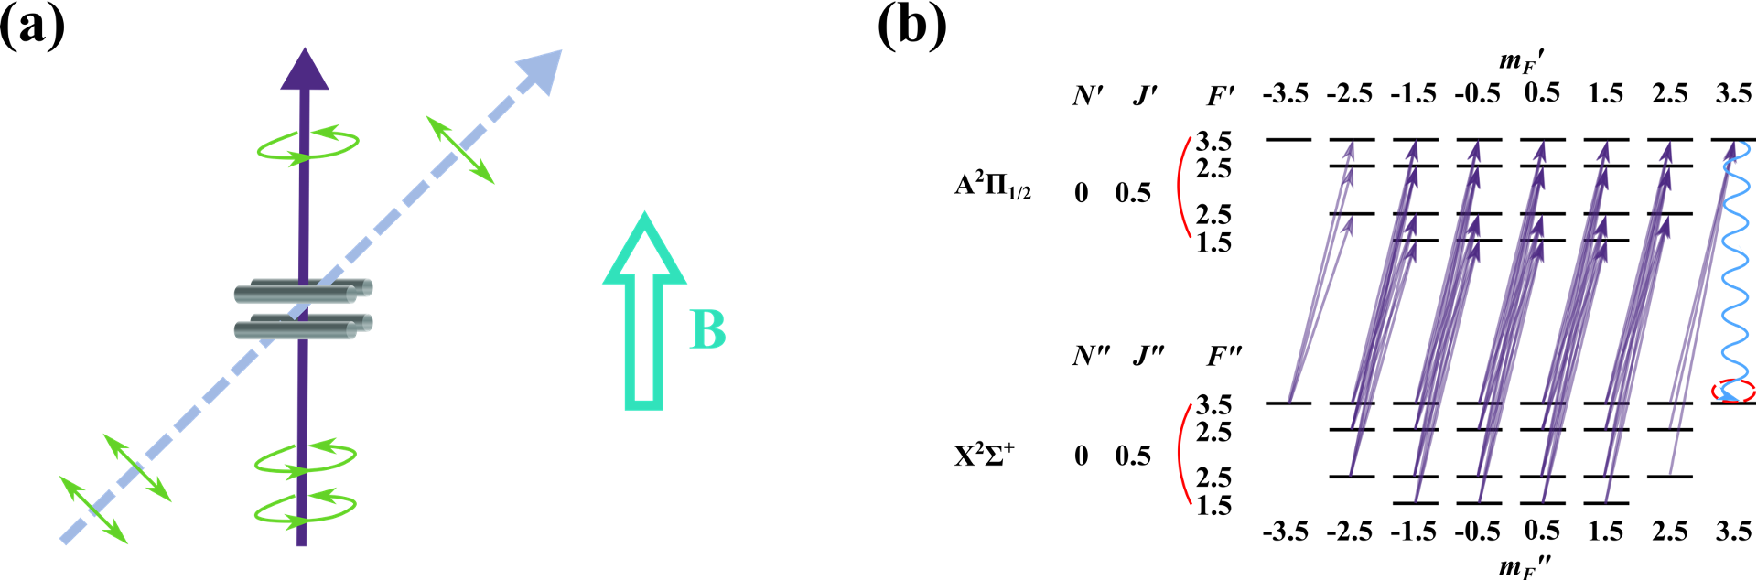
\includegraphics[width=14cm]{schematic_setup}
 \caption{(a) The schematic setup and (b) the hyperfine structure of the rovibrational ground state of $\mathrm{X}^2\Sigma^+$ and $\mathrm{A}^2\Pi_{1/2}$. In (a), rods of a linear Paul trap and two SFFLs are shown. The dashed light blue arrow represents the linearly-polarized SFFL (RC laser) that performs rotational cooling. The solid purple arrow represents the $\sigma^+$-polarized SFFL (HC laser) that drives the $\mathrm{Q}_{11}$(0)-branch transition, optically pumping the population into the stretched hyperfine state in the ground rovibrational manifold. In (b), the hyperfine structure and the set of transitions driven by the $\sigma^+$-polarized SFFL are shown. The population in the rovibrational ground state of $\mathrm{X}^2\Sigma^+$ is driven toward a single dark state, $\lvert \mathrm{X}^2\Sigma^+,\, v=0,\, N=0,\, F''=3.5,\, m_{F''}=3.5\rangle$.}
 \label{schematic_setup}
\end{figure*}

\section{Theory and Methods}
\subsection{Rotational Cooling}
Our group has previously demonstrated broadband rotational cooling of $\mathrm{AlH}^+$ using a linearly-polarized SFFL with 100 fs \pp{pulses} centered at 360 nm. The pulses are generated from a frequency-doubled femtosecond laser (Spectra-Physics Mai Tai) with 80 MHz repetition rate, so the pulse spectrum is divided into a frequency comb with 80 MHz spacing between neighboring teeth. Its large bandwidth pumps many rotational transitions simultaneously. We use \pp{frequency-domain pulse shaping} to selectively excite rotational cooling transitions. The vibrational constant is $\sim$ 1600 cm$^{-1}$ for $\mathrm{AlH}^+$, which is large compared to the bandwidth of the SFFL laser ($\sim$ 200 cm$^{-1}$). This permits us to include only $\lvert \mathrm{X}^2\Sigma^+,\, v = 0,1 \rangle$ and $\lvert \mathrm{A}^2\Sigma^+,\, v = 0 \rangle$ states when modeling the population dynamics.\par 

In the electronic ground state of $\mathrm{AlH}^+$, $\mathrm{X}^2\Sigma^+$, the various angular momenta of $\mathrm{AlH}^+$ are well-described by Hund's case (b), with good quantum numbers  $\left\lbrace\right.\! \Lambda, N,\, S,\, J,\, \pm \!\left.\right\rbrace$. The $\mathrm{A}^2\Pi$ electronic state of $\mathrm{AlH}^+$ is better-described using the Hund's case (a) basis of $\left\lbrace\right.\! \Lambda,\, S,\, \Sigma,\, J, \Omega,\, \pm \!\left.\right\rbrace$. Though $N$ is not a good quantum number in $\mathrm{A}^2\Pi$, for convenience, we still use $N$ to denote different $J$ values in the $\mathrm{A}^2\Pi$ state (see Figure \ref{level_diagram_parity}) and to label transition branches. It should be noted that the rotational states of both the $\mathrm{X}$ and $\mathrm{A}$ states of $\mathrm{AlH}^+$ have parity doublets. In the $\mathrm{X}$ state, the doubling is a result of the interaction of the electron-spin and molecular rotation while the doubling in the $\mathrm{A}^2\Pi$ state is produced by $\Lambda$ doubling. For both electronic states, $v$ is the vibrational quantum number. We invoke the convention that $v'$ ($v''$) denotes the vibrational quantum number of the upper (lower) state.

As shown in Figure \ref{level_diagram_parity}, the rotational cooling process has two parts. The first part is a fast cycle in which linearly-polarized 360 nm pulses of the SFFL drive the electronic transition connecting $\lvert \mathrm{X}^2\Sigma^+,\, v''=0\rangle$ and $\lvert \mathrm{A}^{2}\Pi_{1/2},\, v'=0\rangle$. Following excitation to the $\mathrm{A}$ state, electronic spontaneous emission without vibrational excitation occurs with a relaxation time of $\sim$0.4 \si{\micro}s.  Before rotational cooling, there are significant rotational populations is in the lowest ten rotational states. Through the fast cycle, nearly all of it can be driven into the two lowest rotational states, $\lvert v''=0,\, N''=0,1\rangle$, within a few microseconds. However, the parity is flipped for a dipole transition such as $\lvert \mathrm{A}^2\Pi\rangle$ \pp{--} $\lvert \mathrm{X}^2\Sigma^+\rangle$. As a result, the population in $\lvert \mathrm{X}^2\Sigma^+,\, v''=0,\, N''=1, -\rangle$ cannot be transferred to the rovibronic ground state, $\lvert \mathrm{X}^2\Sigma^+,\, v''=0,\, N''=0,\, +\rangle$ via this fast electronic-cooling cycle which always conserves the parity after an even number of transitions. Nonetheless, the population in $\lvert \mathrm{X}^2\Sigma^+,\, v''=0,\, N''=1, -\rangle$ can still transfer to the $\lvert \mathrm{X}^2\Sigma^+,\, v''=0,\, N''=0,\, +\rangle$, but must do so in an odd number of transitions to flip the parity. The shortest parity-flipping process happens in three transitions: first, the population in $\lvert \mathrm{X}^2\Sigma^+,\, v''=0,\, N''=1, -\rangle$ is excited by the SFFL to the $\mathrm{A}$ state; then there is spontaneous decay to an intermediate state with negative parity, $\lvert \mathrm{X}^2\Sigma^+,\, v''=1,\, N''=1,\, -\rangle$; last, the population undergoes a vibrational relaxation to reach $\lvert \mathrm{X}^2\Sigma^+,\, v''=0,\, N''=0,\, +\rangle$. This parity-flipping process, which constitutes the second part of the cooling process, is relatively slow because the vibrational relaxation time for the $\lvert \mathrm{X}^2\Sigma^+,\, v=1\rangle \rightarrow \lvert \mathrm{X}^2\Sigma^+,\, v=0\rangle$ transition is 140 ms.\par

In our laboratory, $\mathrm{AlH}^+$ ions are trapped in a linear Paul trap and initially sympathetically cooled to sub-Kelvin translational temperatures using co-trapped Doppler-cooled $\mathrm{Ba}^+$. To remove the dark states of the barium ion during the Doppler cooling process, a 2 G magnetic field is applied. After translational cooling, the linearly-polarized SFFL (with polarization of 45$^{\circ}$ relative to the direction of the laboratory-applied magnetic field) is turned on to rotationally cool the molecules into their rovibronic ground state.\par

Rotational cooling of the negative-parity populations is rate-limited by the vibrational-decay timescale. We propose to address this bottleneck through the addition of a 6.7 \si{\micro}m continuous-wave laser which couples the $\lvert \mathrm{X}^2\Sigma^+,\, v''=1,\, N''=1,\, -\rangle$ \pp{--} $\lvert \mathrm{X}^2\Sigma^+,\, v''=0,\, N''=2,\, +\rangle$ transition \pp{to} accelerate part of the parity-flipping process. This technique has not been previously proposed to speed up rotational cooling using broadband lasers. We simulate the rotational cooling process and show that it is accelerated by the addition of the 6.7 \si{\micro}m continuous-wave laser. The simulation results are summarized in Figure \ref{RC_RCV10} and Table \ref{RC_RC_V10table}.


\subsection{Hyperfine Cooling}
As we are interested in pumping our system to a single hyperfine quantum state, we also add a circularly-polarized 360 nm beam. By taking advantage of the selection rules for transitions driven by $\sigma^+$-polarized light, we can optically pump the system to a stretched hyperfine state in which the total angular momentum ($F$) has the largest projection ($m_F$) along the quantization axis. The schematic plot of our setup is shown in Figure \ref{schematic_setup}. When we apply the $\sigma^+$-polarized laser, the selection rule are as follows:

\begin{align*}
\Delta F=0,\, \pm 1 \\
\Delta m_F=1
\end{align*}

As can be seen in Figure \ref{schematic_setup}, if we set the $\sigma^+$-polarized laser to drive the $\mathrm{Q}_{11}$(0)-branch transition\footnote[2]{This notation describes the branch in terms of both $N$ and $J$: $^{\Delta N}\Delta J_{ul}$. Note that $N$ is not a good quantum number in $\mathrm{A}^2\Pi$, and simply serves as a convenient label. If $\Delta N = \Delta J$, then the notation uses one letter to mark the type of branch. $u$ and $l$ denote the spin orientations of the upper and lower states of a transition. In our case, the \pp{upper state} could be either $\mathrm{A}^2\Pi_{1/2}$ or $\mathrm{A}^2\Pi_{3/2}$. These states, corresponding to $\lvert \Omega=\Lambda -\frac{1}{2} \rangle$ or $\lvert \Omega=\Lambda +\frac{1}{2} \rangle$, are denoted as $u=1$ and $u=2$, respectively. Analogously, the lower-state, part of the $\mathrm{X}^2 \Sigma^{+}$ manifold, has $S=1/2$. Our convention is that $l=1$ and $l=2$ represent $\lvert J=N+\frac{1}{2} \rangle$ and $\lvert J=N-\frac{1}{2} \rangle$, respectively.}, $\lvert \mathrm{A}^2\Pi_{1/2}, v'=0, N'=0\rangle$ \pp{--} $\lvert \mathrm{X}^2\Sigma^+, v''=0,\, N''=0\rangle$, most of the population in the rovibronic ground state of $\mathrm{X}^2 \Sigma^{+}$ will be further optically pumped to a single stretched hyperfine state, notably the stretched state of maximal $F$. This stretched hyperfine state is a dark state; it cannot absorb any more $\sigma^+$-polarized photons because there is no higher $m_F$-state available within the $\lvert \mathrm{A}^2\Pi_{1/2},\, v=0\,, N=0\rangle$ manifold. Thus the population will accumulate in the stretch state over time. Adding the 6.7 \si{\micro}m continuous-wave laser here also accelerates the hyperfine cooling process since it is dependent upon the rate of rotational cooling. The simulation results are shown in Figure \ref{RCHC_RCHCV10} and Table \ref{RCHC_RCHCV10table}.

\section{Simulation Details}

%\begin{center}
\begin{table*}
\centering
\begin{minipage}[b]{0.45\linewidth}
\renewcommand*{\thempfootnote}{\fnsymbol{mpfootnote}}
\let\TPToverlap=\TPTrlap
\caption{Molecular constants for the $\mathrm{X}^2\Sigma^+$ state of $\mathrm{AlH}^+$\tnote{$\ddag$}}
\begin{threeparttable}
\renewcommand{\arraystretch}{1.25}
\setlength{\tabcolsep}{1em}
\begin{tabular}{lcc}
 \hline
Constant\cite{szajna2011high}     &    $ v=0$   &   $ v=1$    \\
 \hline
$B_{v}$                           &$6.563231$   &$6.184845$    \\   \hline
$D_{v}\times 10^{4}$              &$4.5720$     &$5.0983$      \\ \hline
$H_{v}\times 10^{8}$              &$-0.238$     &$-6.586$       \\ \hline
$L_{v}\times 10^{11}$             &$-1.712$     &               \\ \hline
$M_{v}\times 10^{14}$             &$1.140$      &               \\ \hline
$N_{v}\times 10^{18}$             &$-7.07$      &               \\ \hline
$\gamma_{v}\times 10^{2}$         &$5.665$      &$5.035$        \\ \hline
$\gamma_{Dv}\times 10^{5}$        &$-1.896$     &$-2.09$        \\ \hline
Origin                                          &$0$              &$1523$        \\ 
\hline
\end{tabular}
\begin{tablenotes}
\item[$\ddag$] in $cm^{-1}$
\end{tablenotes}
\end{threeparttable}
\label{Xparameters}

\end{minipage}
\hspace{0.2cm}
\begin{minipage}[b]{0.45\linewidth}
\centering
\let\TPToverlap=\TPTrlap
\caption{Molecular constants for the $\mathrm{A}^2\Pi$ state of $\mathrm{AlH}^+$ \tnote{$\ddag$}}
\renewcommand{\arraystretch}{1.25}
\begin{threeparttable}
\setlength{\tabcolsep}{1em}
\begin{tabular}{lc}
 \hline
Constant                                  &                $ v=0$   \\
 \hline
$B_{v}$                                   &$6.727$ \cite{almy1934band}     \\   \hline
$A_{v}$                                   &$108$ \cite{almy1934band}        \\ \hline
$p_{v}\times 10^{2}$             &$1.643$ \cite{szajna2011high}    \\ \hline
$q_{v}\times 10^{3}$             &$1.499$ \cite{szajna2011high}    \\ \hline
$D_{v}\times 10^{4}$             &$-4.14$ \cite{almy1934band}     \\ \hline
Origin                                      &$27713$ \cite{szajna2011high}   \\ 
\hline
\end{tabular}
\begin{tablenotes}
\item[$\ddag$] in $cm^{-1}$
\end{tablenotes}
\end{threeparttable}
\label{Aparameters}
%\end{table*}
%\end{center}
\end{minipage}
\end{table*}
%\end{center}

\begin{center}
\begin{table*}
\let\TPToverlap=\TPTrlap
\centering
\small
  \captionsetup{justification=centering}
  \caption{Permanent and transition dipole moments ($\langle$ State i $\lvert\,\mu\,\rvert$ State j$\rangle$) \tnote{$\ddag$}}
  \renewcommand{\arraystretch}{1.5}
\begin{threeparttable}
\setlength{\tabcolsep}{3pt}
\begin{tabular*}{0.48\textwidth}{@{\extracolsep{\fill}}cccc}
\hline
\diagbox{State i}{State j} &$\mathrm{X}^2\Sigma^+,\, v=0$ &$\mathrm{X}^2\Sigma^+,\, v=1$    &$\mathrm{A}^2\Pi,\, v=0$  \\ 
\hline
$\mathrm{X}^2\Sigma^+,\, v=0$         &$-0.389$               &                      & \\   \hline
$\mathrm{X}^2\Sigma^+,\, v=1$         &$0.087$                &$-0.2861$             & \\   \hline
$\mathrm{A}^2\Pi,\, v=0$              &$1.566$                &$-0.2806$             &$-0.928$\\ \hline
\end{tabular*}
\begin{tablenotes}
\item[$\ddag$] in debye
\end{tablenotes}
\end{threeparttable}
\label{dipolemoment}
\end{table*}
\end{center}


\begin{table*}[htbp!]
\centering
\let\TPToverlap=\TPTrlap
\captionsetup{justification=centering}
\caption{Hyperfine constants of $\mathrm{AlH}^+$ in terms of Frosch--Foley coefficients and parameters of nuclear quadrupole interaction\tnote{$\ddag$}}
\renewcommand{\arraystretch}{1.5}
\begin{threeparttable}
\setlength{\tabcolsep}{6pt}
\begin{tabular}{*{5}{c}}
\hline
\multirow{2}{*}{Constant} &\multicolumn{2}{c}{$\mathrm{X}^2\Sigma^+$} &\multicolumn{2}{c}{$A^2\Pi$} \\
\cline {2-5}
&Al &H  &Al &H\\
 \hline
a               &\num{1.680E-3}           &\num{8.64E-5}            &\num{8.511E-3}              &\num{5.53E-4}         \\
b               &\num{3.951E-2}           &\num{2.01E-2}             &\num{1.382E-2}             &\num{-9.35E-3}         \\
c               &\num{5.039E-3}          &\num{2.59E-4}             &\num{-5.654E-3}            &\num{2.79E-4}         \\
d               &\num{0}                        &\num{0}                         &\num{1.040E-2}             &\num{4.60E-4}          \\
$eQq_0$    &\num{-1.341211E-3}    &\num{2.12636E-6}        &\num{6.20358E-4}       &\num{2.34231E-6}      \\
$eQq_2$    &\num{0}                        &\num{0}                          &\num{-2.89652E-3}    &\num{-5.63315E-7}     \\               
\hline
\end{tabular}
\begin{tablenotes}
\item[$\ddag$] in cm$^{-1}$
\end{tablenotes}
\end{threeparttable}
\label{hyperfineconstant}
\end{table*}

Our population dynamics were modeled by the following system of rate equations:
\begin{align}
\begin{aligned}
\frac{\partial\rho_i}{\partial t}=-\sum_{j\neq i}B_{ij}(I_{\mathrm{BBR}}+I_{\mathrm{laser}})\rho_i - \sum_{j<i}A_{ij}\rho_i \\
+\sum_{j\neq i}B_{ji}(I_{\mathrm{BBR}}+I_{\mathrm{laser}})\rho_i + \sum_{j>i}A_{ji}\rho_i 
\end{aligned}
\end{align}
where $\rho_i$ is the population fraction in state $i$. The initial population is assumed to be thermal with a temperature of 300 K. $I_{\mathrm{BBR}}$ and $I_{\mathrm{laser}}$ are the energy densities of the blackbody radiation and laser. $A$ and $B$ are the spontaneous emission and stimulated emission Einstein coefficients, respectively.
\begin{align}
\begin{aligned}
A_{ul} &= \frac{2\pi \widetilde{\nu}^2 q_e^2}{\epsilon_0 m_e c} \frac{g_l}{g_u} f_{lu}\\
B_{ul} &= \frac{q_e^2}{4 \epsilon_0 m_e h c \widetilde{\nu}} \frac{g_l}{g_u} f_{lu} \\
B_{lu} &= \frac{q_e^2}{4 \epsilon_0 m_e h c \widetilde{\nu}} f_{lu}\\
\end{aligned}
\end{align}
In order to determine the Einstein coefficients using Equation (2), we utilized Western's PGOPHER\cite{western2017pgopher} software to compute transition energies and oscillator strengths for $\mathrm{AlH}^+$. \pp{A 10 G laboratory-frame magnetic field was assumed to address the problem of the dark states while driving the P-branch rotational cooling transition with a linearly-polarized beam. By adding the 10 G magnetic field with an angle of 45$^{\circ}$ with respect to the polarization direction of the rotational cooling laser (see Figure \ref{schematic_setup}), dark state evolves on the time scale of Larmor precession (10$^9$ s$^{-1}$), which is sufficiently fast compared to the Rabi frequency of the rotational cooling laser (10$^8$ s$^{-1}$) to decrease the population accumulation in the dark state.}

We required a number of empirical parameters that describe the states of the $\mathrm{AlH}^+$. Table \ref{Xparameters} and \ref{Aparameters} present the empirical values used throughout this work to describe the $\mathrm{X}^2 \Sigma^{+}$  and $\mathrm{A}^2\Pi$ states.

Additionally, we used Le Roy's LEVEL\cite{le2017level} to calculate the electric permanent and transition dipole-moments from potential-energy and transition dipole-moment functions of a prior work\cite{nguyen2011challenges}. These results are presented in Table \ref{dipolemoment}.

Dalton\cite{daltonpaper, daltonwebpage} quantum computational software was used to compute hyperfine and nuclear-quadrupole coupling constants of the $\mathrm{X}^2\Sigma^+$ and $\mathrm{A}^2\Pi$ states. We chose the pcJ-1 basis set because pcJ family was developed for RMN/EPR spin-spin coupling constants and has tight functions that are well-suited for describing the electron density near the nucleus. Density Functional Theory (DFT) using the B3LYP density functional was applied with an pcJ-1 basis set for all computations.

\pp{For the spin-dipolar interaction coupling constants, Dalton gives the values of the hyperfine tensor components ($A_{xx},\, A_{yy},\, A_{zz}$) and the Fermi contact term ($A_{iso}$), while Pgopher requires the input of hyperfine constants in terms of Frosch--Foley coefficients ($a$, $b$, $c$ and $d$). The conversion formulas are listed as follows.}

\pp{\begin{align}
\label{eqn:spin-dipolar}
\begin{aligned}
  c &= \frac{3}{2} A_{zz} \\
  d &= A_{xx}-A_{yy} \\
  b &= A_{iso}-\frac{c}{3} \\
  a &= d + \frac{c}{3}
\end{aligned}
\end{align}}

\pp{For the nuclear quadrupole coupling constants, we used the electric field gradients ($q_{xx}\equiv \partial ^{2}V_{x}/\partial x^{2}$, $q_{yy}\equiv \partial ^{2}V_{y}/\partial y^{2}$, $q_{zz}\equiv \partial ^{2}V_{z}/\partial z^{2}$ in $\mathrm{MHz}$) and nuclear electric quadrupole moment ($Q$ in barn) output from Dalton to calculate $eQq_0$ and $eQq_2$ (both in $\mathrm{cm^{-1}}$) required by Pgopher. The formulas are given by}

\pp{\begin{align}
\label{eqn:nuclear-quadrupole}
\begin{aligned}
  eQq_0 &= 234.96478\cdot 10^6\cdot c^{-1}\cdot q_{zz} Q \\
  eQq_2 &= 234.96478\cdot 10^6\cdot c^{-1}\cdot (q_{xx}-q_{yy}) Q \\
\end{aligned}
\end{align}}

\pp{where c is the speed of light ($=29979245800$ $\mathrm{cm}$). The input hyperfine coupling constants for Pgopher are listed in Table \ref{hyperfineconstant}.}

At room temperature, 99$\, \%$ of the $\mathrm{AlH}^+$ population is in the lowest vibrational state, $v=0$, within the $\mathrm{X}^2 \Sigma^+$ manifold. In turn, within this vibrational ground state, thermal distribution produces significant populations among the first ten $J$-levels, $J=0.5$--$9.5$, and less than 4$\, \%$ in $J>9.5$. Therefore, we included only these lowest ten $J$-states in our \pp{rate equation simulation} for both the $\mathrm{X}$ and $\mathrm{A}$ states. We also included the $\mathrm{X}^2\Sigma^+ (v''=1)$ manifold so that we can simulate the parity-flipping process via the intermediate state, $\lvert \mathrm{X}^2\Sigma^+,\, v''=1,\, N''=1, -\rangle$.

Our femtosecond laser has a frequency-domain representation in the simulation. The spectrum was described by 80 MHz-spaced comb teeth within a Gaussian envelope of $\sim$ 7 nm FWHM bandwidth and centered at 360 nm. We modeled our pulse shaping apparatus as a cut-off filter to the laser spectrum. The cut-off frequency was chosen so as to pass the range of frequencies that selectively drives a set of rotational cooling transitions. For example, we chose to drive the $\mathrm{P}_{11}$, $\mathrm{^OP}_{12}$ and the $\mathrm{^PQ}_{12}$ branches using the linearly-polarized SFFL and then include the $\mathrm{Q}_{11}(0)$ branch for the $\sigma^+$-polarized SFFL. We assumed a 200 mW power split equally between the linear- and the $\sigma^+$-polarized beams with a focused 400 \si{\micro}m-diameter spot at the position of $\mathrm{AlH}^+$ molecules.

The typical optical transition linewidth for $\mathrm{AlH}^+$ is $\sim$ 20 MHz, which is smaller than the 80 MHz comb-teeth spacing of the femtosecond laser spectrum. As a result, it is possible for the SFFL comb-line to fall outside of the transition linewidths of some of the transitions we desired to drive. We solved this issue in the simulation by introducing a Doppler-broadened linewidth contribution that assumed $\sim$1 K translational temperature for the $\mathrm{AlH}^+$ ion cloud. Doing so ensured that there was at least one comb-line within the linewidth of every desired cooling transition. One can accomplish this form of broadening in the experiment by raising the translational temperature of the $\mathrm{AlH}^+$ ions in a couple ways. One can excite the secular motion of the $\mathrm{AlH}^+$ with an AC field or introduce additional micro-motion by shifting the entire ion cloud away from the geometric center of the Paul trap using a DC field. After internal cooling is finished, one can then turn off the source of translational heating, allowing the $\mathrm{AlH}^+$ to be sympathetic cooled once again by the laser-cooled $\mathrm{Ba}^+$.

\begin{figure*}[htbp!]
  \centering
  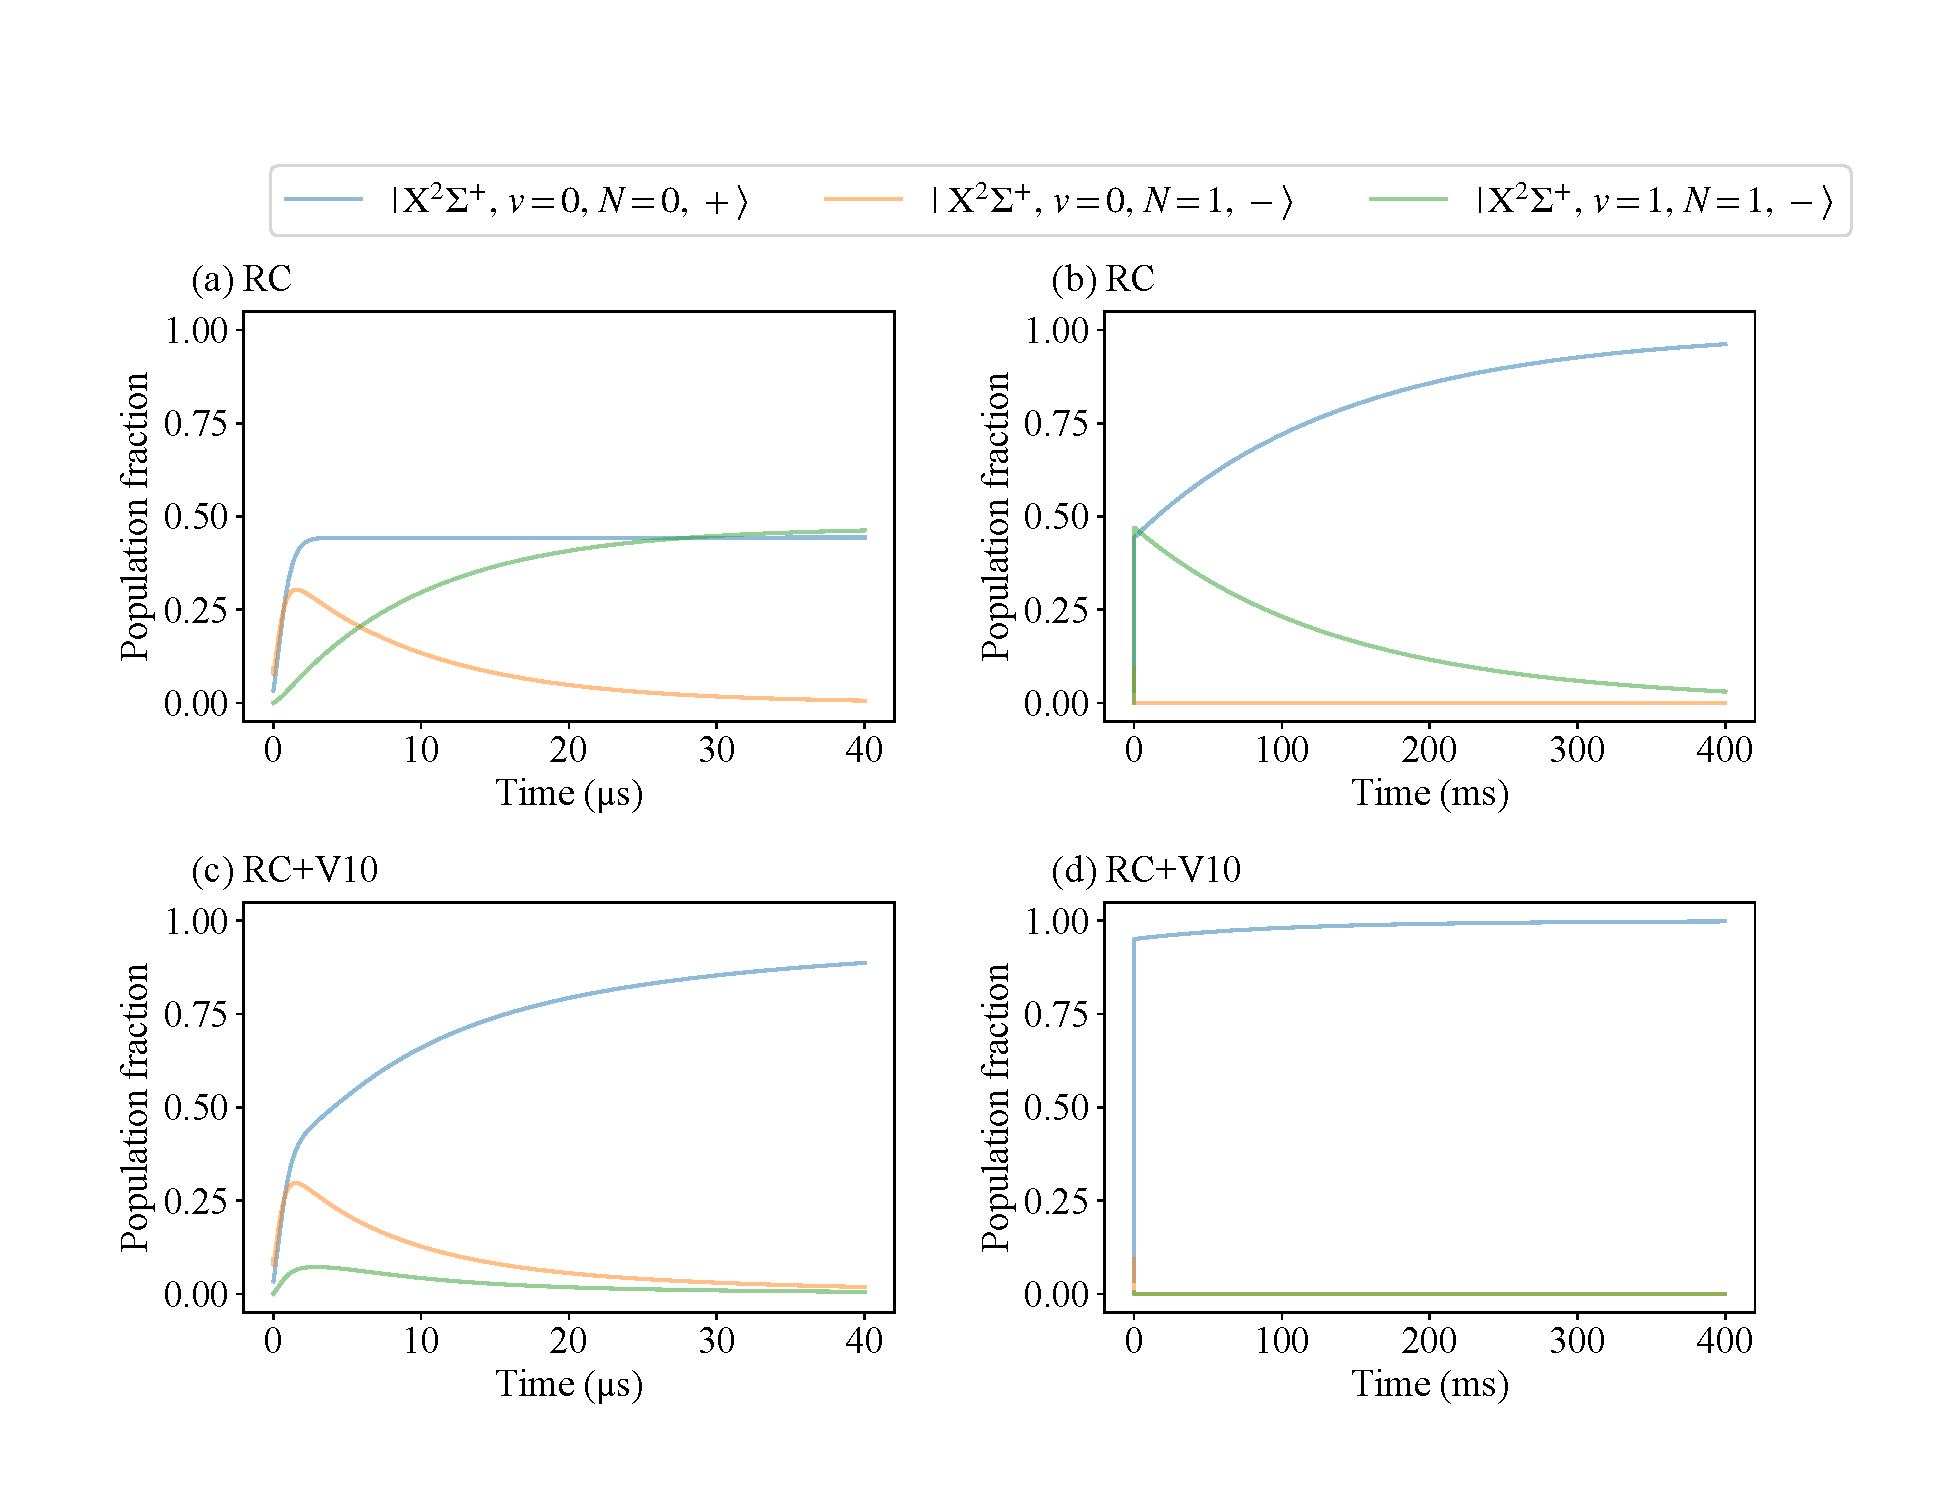
\includegraphics[width=11cm]{RC_RCV10}
  \caption
  {Simulated population dynamics for rotational cooling: The top two plots are for the cases in which only the linearly-polarized rotational cooling SFFL (RC) was applied for (a) 40 \si{\micro}s and (b) 400 ms, respectively. The bottom two plots describe rotational cooling via the SFFL and the additional laser (V10) to drive the $\lvert \mathrm{X}^2\Sigma^+,\, v''=1,\, N''=1,\; - \;\rangle$ \pp{--} $\lvert \mathrm{X}^2\Sigma^+,\, v''=0,\, N''=2,\, +\rangle$ transition, for (c) 40 \si{\micro}s and (d) 400 ms, respectively.
  }\label{RC_RCV10}
\end{figure*}

\begin{figure*}[htbp!]
  \centering
  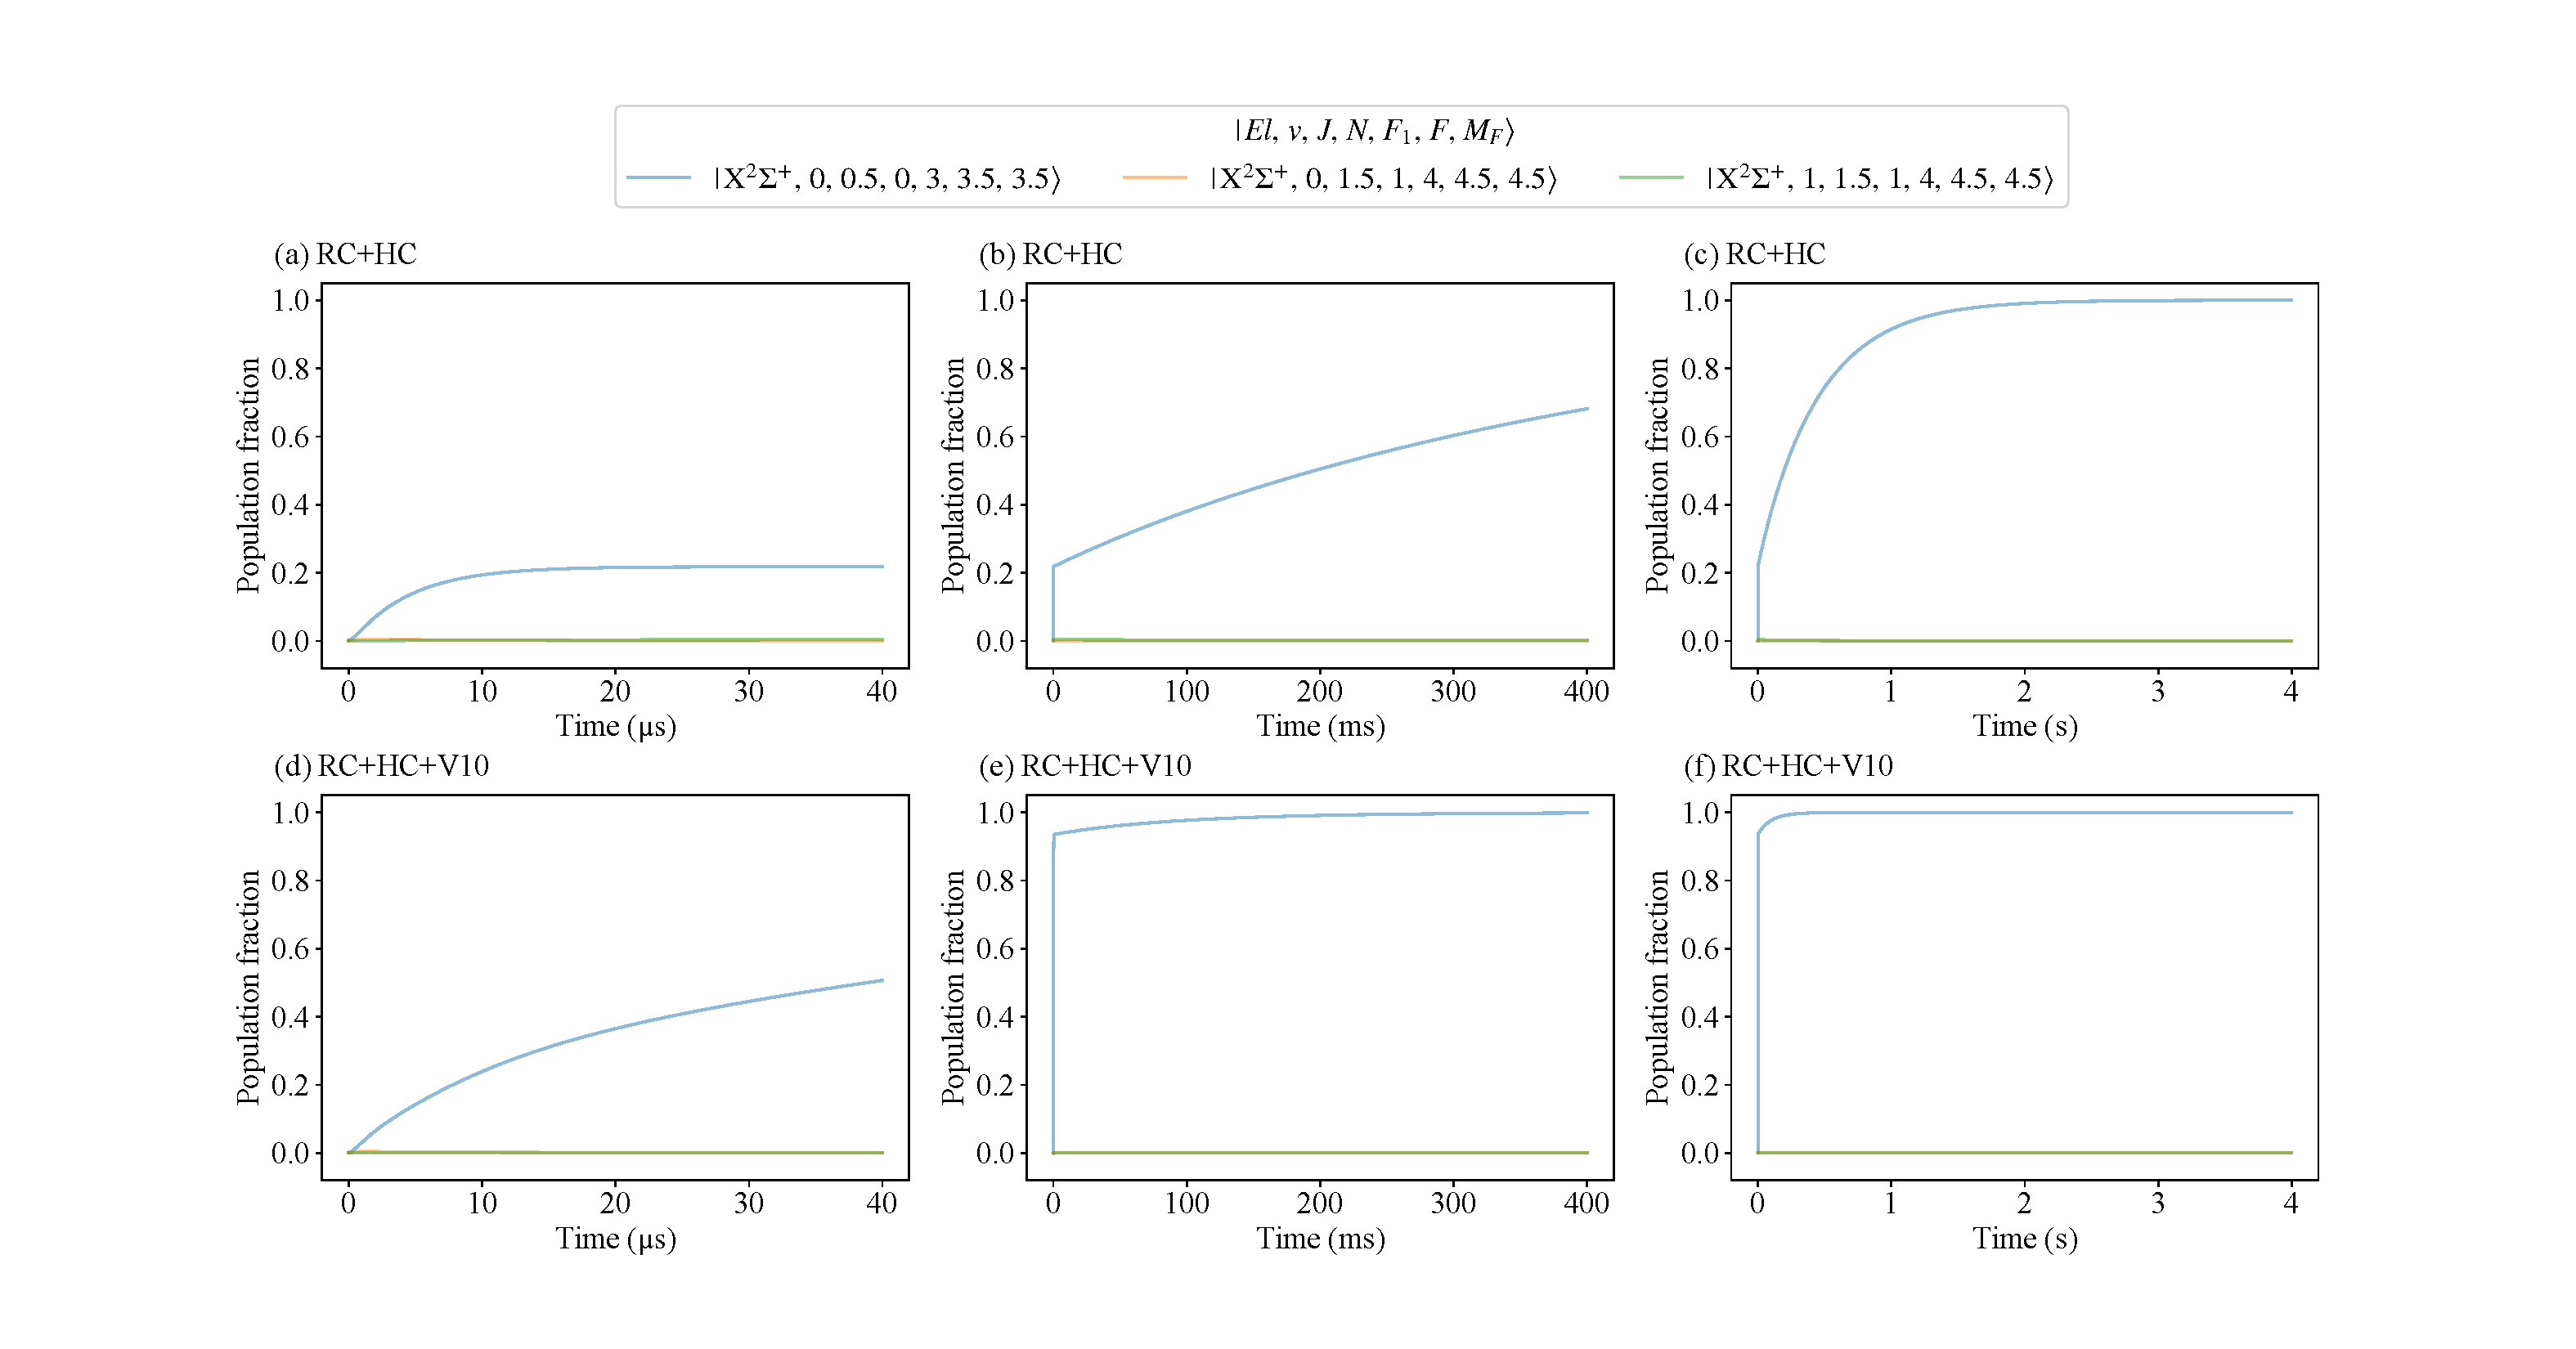
\includegraphics[width=16.5cm]{RCHC_RCHCV10}
  \caption
  {Simulated population dynamics for preparation of a single hyperfine state: The top three plots are for the cases in which the linearly-polarized rotational cooling SFFL (RC) and the $\sigma^+$-polarized hyperfine-cooling SFFL (HC) were applied for (a) 40 \si{\micro}s, (b) 400 ms, and (c) 4 s, respectively. The bottom two plots describe \pp{rotational and hyperfine cooling} via the linearly- and circularly-polarized SFFLs and the additional laser (V10) to drive the $\lvert \mathrm{X}^2\Sigma^+,\, v''=1,\, N''=1,\, -\rangle$ \pp{--} $\lvert \mathrm{X}^2\Sigma^+,\, v''=0,\, N''=2,\, +\rangle$ transition, for (d) 40 \si{\micro}s, (e) 400 ms, and (f) 4 s, respectively.
}\label{RCHC_RCHCV10}
\end{figure*}

\begin{table*}[!htbp]
\begin{minipage}[b]{0.45\linewidth}
\centering
\renewcommand{\arraystretch}{1.25}
\caption{The time for the rovibronic ground state population (p$_{0}^\mathrm{R}$) to reach $63$ $\%$ and $95$ $\%$.}
\setlength{\tabcolsep}{6pt}
\begin{tabular}{ccc}
%\hline
%\multicolumn{3}{|c|}{WTmetaD parameters} \\
\hline
Laser fields & $63$ $\%$ &  $95$ $\%$   \\ 
\hline
RC & $60.0$ ms & $359.4$ ms \\ \hline
RC, V10 & $8.7$ \si{\micro}s & $162.0$ \si{\micro}s \\ 
\hline
\end{tabular}
\label{RC_RC_V10table}

\end{minipage}
\hspace{0.2cm}
\begin{minipage}[b]{0.45\linewidth}
\centering
\renewcommand{\arraystretch}{1.25}
\caption{The time for the hyperfine stretched state population (p$_{0}^\mathrm{H}$) to reach $63$ $\%$ and $95$ $\%$.}
\setlength{\tabcolsep}{6pt}
\begin{tabular}{ccc}
%\hline
%\multicolumn{3}{|c|}{WTmetaD parameters} \\
\hline
Laser fields & $63$ $\%$ &  $95$ $\%$   \\ 
\hline
RC, HC &$334.6$ ms & $1240$ ms \\ \hline
RC, HC, V10 & $67.6$ \si{\micro}s & $25.4$ ms \\
\hline
\end{tabular}
\label{RCHC_RCHCV10table}
\end{minipage}
\end{table*}

We simulated the laser-enhanced parity-flipping processes as well. For such cases, we represented the laser (V10) that drives the $\lvert \mathrm{X}^2\Sigma^+,\, v''=1,\, N''=1,\, -\rangle$ \pp{--} $\lvert \mathrm{X}^2\Sigma^+,\, v''=0,\, N''=2,\, +\rangle$ transition to match the specifications of a commercial Fabry-Perot quantum-cascade laser from Thorlabs. This laser outputs $\sim$ 200 mW with $\sim$15 cm$^{-1}$ bandwidth and could be customized to center at $\sim$ 6.7 \si{\micro}m to drive the transition of the $v'=1$  \pp{--} $v''=0$ band in the electronic ground state of $\mathrm{AlH}^+$.

\section{Result and discussion}
Figure \ref{RC_RCV10} and Table \ref{RC_RC_V10table} present rotational cooling rates for two schemes. In the first scheme, we apply the linearly-polarized rotational cooling laser (RC). In the second scheme, we apply the rotational cooling laser (RC) as well as a laser (V10) that drives the $\lvert \mathrm{X}^2\Sigma^+,\, v''=1,\, N''=1,\, -\rangle$ \pp{--}  $\lvert \mathrm{X}^2\Sigma^+,\, v''=0,\, N''=2,\, +\rangle$ transition. From Figure \ref{RC_RCV10}(a), it can be seen that without the V10 laser, the population in the rovibrational ground state ($v$,\,$N$) = (0,0) increases to 45 $\%$ within a few microseconds through the fast rotational cooling cycle. Afterwards, the population in (0,0) continues to increase but with a slower rate as shown in Figure \ref{RC_RCV10}(b). This behavior can be attributed to two time scales. At shorter times, population accumulates in the $\lvert \mathrm{X}^2\Sigma^+,\, v''=0,\, N''=1,\, -\rangle$ state after it undergoes a parity flip via the $\lvert \mathrm{X}^2\Sigma^+,\, v''=1,\, N''=1,\, -\rangle$ state.  At longer times, vibrational relaxation (140 ms decay constant) starts to dominate the process. The addition of the V10 laser effectively outcompetes the vibrational relaxation between $\lvert \mathrm{X}^2\Sigma^+,\, v''=1,\, N''=1,\, -\rangle$ and $\lvert \mathrm{X}^2\Sigma^+,\, v''=0,\, N''=2,\, +\rangle$. The time it takes for the population in the rovibronic ground state, p$_{0}^\mathrm{R}$, to grows to 63 $\%$ reduces from 60.0 ms to 8.7 \si{\micro}s. The trend continues as p$_{0}^\mathrm{R}$ reaches 95 $\%$, which takes only 162.0 \si{\micro}s, also significantly shorter than the 359.4 ms required in the absence of the V10 laser.

The Transfer of population among hyperfine states was demonstrated in Ref.[14] with HD$^{+}$. The transfer took tens of seconds with the target population only \pp{increasing} a few percent. In this work, we propose a more efficient \pp{mean} of hyperfine-cooling, again using $\mathrm{AlH}^{+}$ as the system. Figure \ref{RCHC_RCHCV10} and Table \ref{RCHC_RCHCV10table} present our simulation results for two hyperfine-cooling schemes. In the first scheme, we apply the rotational cooling laser (RC) and the $\sigma^+$-hyperfine-cooling laser (HC). For the second scheme, in addition to the RC and HC lasers, we apply the rovibrational coupling laser (V10). As can be seen in Figure \ref{RCHC_RCHCV10}(a), in the absence of the V10 laser, the population in the stretched hyperfine state increases to $\sim 20 \%$ during the first tens of microseconds via the fast rotational cooling cylce and the hyperfine optical pumping cycle. Since the hyperfine cooling process takes additional cycles to transport the population to the stretched state, the time scale is longer when compared to the case during which only the RC laser is applied. \pp{The transfer rate eventually slows down due to the relatively long vibrational relaxation time scale}. After one second, the population reaches more than 90 $\%$. From Figure \ref{RCHC_RCHCV10}(d), we can see that when the V10 laser is also applied, the impact of vibrational relaxation is mitigated. The time it takes for the stretched hyperfine-state population in the rovibronic ground state, p$_{0}^{\mathrm{H}}$, to reach 63 $\%$ is shortened from 334.6 ms to 67.2 \si{\micro}s. If we leave the lasers on, p$_{0}^{\mathrm{H}}$ can reach 95 $\%$ in 25.4 ms with the V10 laser, a near 50-fold reduction from the 1240 ms \pp{in its absence}. 

\section{Conclusions}
In order to take full advantage of molecular ions, efficient and precise state preparation is important. We have described a method to achieve faster and more selective internal state cooling in the molecular ion, $\mathrm{AlH}^+$. We based our design on the simple premise that in order to speed up the cooling process, we have to accelerate the rate-limiting step. In the $\mathrm{AlH}^+$ system, the rate-limiting step is the parity-flipping process. We expect to accomplish this task by adding a new laser field that drives population out of the intermediate state. We further describe an extension to our previous rotational cooling work that should enable one to drive population to a single hyperfine state. We exploit the selection rules of a circularly-polarized laser field and show by simulation that we should be able to drive 95 $\%$ of an ensemble of $\mathrm{AlH}^+$ molecules to a single quantum state in about one second. 

\section*{Conflicts of interest}
In accordance with our policy on \href{http://www.rsc.org/journals-books-databases/journal-authors-reviewers/author-responsibilities/#code-of-conduct}{Conflicts of interest} please ensure that a conflicts of interest statement is included in your manuscript here.  Please note that this statement is required for all submitted manuscripts.  If no conflicts exist, please state that ``There are no conflicts to declare''.

\section*{Acknowledgements}
The Acknowledgements come at the end of an article after Conflicts of interest and before the Notes and references.

%%%END OF MAIN TEXT%%%

%The \balance command can be used to balance the columns on the final page if desired. It should be placed anywhere within the first column of the last page.

\balance

%If notes are included in your references you can change the title from 'References' to 'Notes and references' using the following command:
%\renewcommand\refname{Notes and references}

%%%REFERENCES%%%
\bibliography{AlH+_references.bib} %You need to replace "rsc" on this line with the name of your .bib file
\bibliographystyle{rsc} %the RSC's .bst file

\end{document}
